
\documentclass[headsepline,12pt,a4paper]{scrartcl}
% Helvetica
\renewcommand{\rmdefault}{cmss}
\usepackage[scaled=0.95]{helvet}

\usepackage[utf8]{inputenc} % Bei Windowssystemen: ansinew; Apple: applemac
\usepackage[T1]{fontenc}
%\usepackage{german}
\usepackage{hyperref}
\usepackage{amsmath,amssymb,amsfonts,latexsym} % zusaetzliche math. Symbol- und Schriftpakete
\usepackage{scrpage2} % schöne Kopf- und Fußzeilen
\usepackage{enumerate}
\usepackage{stmaryrd}
\usepackage{bbm}
\usepackage{graphicx}
\usepackage{amssymb}
\usepackage{multicol}
\usepackage{color}
\usepackage{listings}
\typearea{12}


%% Eigene Varianten zum Code integrieren
%%\renewcommand\lstlistlistingname{Quellcodeverzeichnis}
\definecolor{darkblue}{rgb}{0,0,.6}
\definecolor{darkred}{rgb}{.6,0,0}
\definecolor{darkgreen}{rgb}{0,.6,0}
\definecolor{red}{rgb}{.98,0,0}

\lstset{language=C,alsolanguage=Matlab,frame=shadowbox,frameround=tftf,captionpos=b,tabsize=4,escapechar=\$,
					basicstyle=\scriptsize\ttfamily,
					keywordstyle=\color{darkblue}\bfseries\ttfamily,
					stringstyle=\ttfamily\color{darkred},  
					commentstyle=\itshape\color{darkgreen},
					xleftmargin=.52cm,
					xrightmargin=.52cm}
	\renewcommand\lstlistlistingname{Quellcodeverzeichnis}	


%% Eigene itemizevarmit kleinem zeilenabstand
\newenvironment{myitemize}{\begin{enumerate}\itemsep -5pt}{\end{enumerate}}
\newenvironment{aenumerate}{\begin{enumerate}[a)]}{\end{enumerate}}
\newenvironment{myvector}{\left ( \begin{array}{*{1} {c}}}{\end{array}\right )}

%% Kopf- und Fußzeilen
\pagestyle{scrheadings}

\ohead[\pagemark]{\today\quad Seite \pagemark\\}
\automark[section]{section}
\lohead[\textbf{\headmark}]{\textbf{Feature Selection\\Johannes Schöllhorn, Julian Schwab, Dennis Schwartz}}
\chead[]{Users Manual\\}
\lefoot[]{}
\rofoot[]{}
\refoot[]{}
\lofoot[]{}
\cfoot[]{}
\rehead{\textbf{}}

\setheadsepline{0.5mm}
\setfootsepline{0mm}

\linespread {1.25}
\setlength{\parindent}{0mm}

% no section numbering
\setcounter{secnumdepth}{0}



\begin{document}
\pagenumbering{arabic}
\begin{titlepage}
  \author{Johannes Schöllhorn, Julian Schwab, Dennis Schwartz}
  \title{Feature Selection - User Guide}
  \date{\today}
  \maketitle
\end{titlepage}


\tableofcontents

\newpage

\section{Input Format}

At the moment the csv format is used for data input. The csv file has some format conventions listed here :

\begin{itemize}
\item The class of a dataset has to be in the second column
\item The decimal mark has to be a point ('.')
\item There should be no thousands separator 
\end{itemize}

The delimiter of columns in the csv file is comma ',' per default, but the program will ask for the delimiter, if comma does not lead to the correct format.\\
The symbols or strings for the different classes do not matter, however it should be limited to two different classes in one file (because of binary classification).

An example, how a correct input should look like (here the classes are named 1 and 0): \\ \\
\begin{tabular}[h]{| c | c | c | c |}
  \hline
name & class & feature 1 & feature 2 \\
\hline
col 1 & 1 & 1.00 & 23.345 \\
\hline
col 2 & 0 & -45.34 & 1.34 \\
\hline
\end{tabular} \\
 
in a .csv-file this would look like this : \\

name, class, feature 1, feature 2\\
col1, 1, 1.00, 23,345\\
col2, 0, -45.34, 1.34\\


\section{Programm Parameters}

The feature selection has varoius parameters to choose.
\subsection{Wrapper}
There are two different wrapper types implemented in this software. A
forward selection wrapper and EvA2. 

\subsubsection{Forward Selection}
The forward selection wrapper starts with an empty set of features and
will add one feature per iteration, choosing whichever feature improves the performance the most. When performance improvement stagnates over a certain
time period, the wrapper stopps.
\subsubsection{EvA2}
EvA2
\footnote[1]{\url{http://www.ra.cs.uni-tuebingen.de/software/JavaEvA/introduction.html}}
is a workbench of evolutionary algorithms released by the University of
Tuebingen. The algorithm forms populations of feature subsets
(individuals). As in a biological system the individuals can mutate or couple. The fitness of an individual is defined by the performance of its feature subset.



\subsection{Performance}
At this state of development, the program has implemented two different ways to compute the performance which is defined by the success of binary classification. Both ways use a confusion matrix  as input which is calculated by the cross validation. This matrix is computed by evaluating the predictions of the classifier as follows : \\
\begin{enumerate}
\item [TP] A true positive will be counted if both the actual class of a sample (as given in the input file) and its predicted class are true.
\item [FN] A false negative will be counted if the actual class of a sample is true but its predicted class is false.
\item [FP] A false positive will be counted if the actual class of a sample is false but its predicted class is true .
\item [TN] A true negative will be counted if both the actual class of a sample and its predicted class are false.
\end{enumerate}

\subsubsection{Matthews Correlation Coefficient}
The Matthews correlation coefficient is computed using the following formula \footnote[2]{\url{http://en.wikipedia.org/wiki/Matthews_correlation_coefficient}} :

  \[MCC = \frac{TP \cdot TN - FP \cdot FN}{\sqrt{(TP + FP) (TP + FN) (TN + FP) (TN + FN)}}\]

The performance is measured between $-1$ and $1$. $-1$ is the worst
performance, with no class predicted correctly and $1$ is the best, where all predictions of the classifier are correct.

\subsubsection{Accuracy}
Accuracy computes the percentage of correct predictions by the classifier. \\
Accuracy is calculated using the following formula\footnote[3]{\url{http://en.wikipedia.org/wiki/Accuracy_and_precision}} : 
\[ accuracy = \frac{TP + TN}{TP + FP + FN + TN} \]

If the accuracy is 0, 0 \% of the predictions are correct, if it is 1 every prediction is correct.

\subsection{Classifier}
At this state the only implemented classifier is the CSVC-Classifier by libSVM\footnote[4]{\url{http://www.csie.ntu.edu.tw/~cjlin/libsvm/}} using a linear kernel.

\subsection{Cross validation}
Cross validation is a statistical technique to evaluate the quality of the classifiers predictions. \\
In $k$-fold cross validation the data will be split in k subsets(folds) of which one will be used to perform the prediction on, while the remaining subsets will be used to validate said prediction.\\ The number of subsets used may have an impact on the results as well as on computational time. It can be set to anything from 2 (2-fold), up to the number of samples in the given data (leave-one-out). \\
For example: If you want to use a 2-fold cross validation, set $k = 2$. If you want to choose leave-one-out, set $k$ to the number of samples in your input.

\section{Console Usage}
It is possible to run the program via console, but its usage will set limitations to output capabilities. At this stage there is no save function for the intermediate and final results, as well as the plot depicting the improving performance of a run.\\

To use the program in a shell or console run ConsoleClient.java. \\
There are multiple ways to start a run using the console client:
\begin{enumerate}
\item 
Entering consoleclient -i will start an interactive console client showing a dialogue, asking for parameters. You will have to enter parameters step by step.
\item 
Entering consoleclient [file] will run the program using default parameters.\\
Parameters per default are set to:
\begin{itemize}
\item wrapper : Forward selection
\item performance : MCC
\item cross validation : 2-fold cross validation
\item classifier : CSVC
\end{itemize}
\item 
If you enter consoleclient [file] and you want to choose different
parameters, these are the options to choose from:
\begin{itemize}
\item wrapper:
enter FWD (Forward selection) or EVA (Eva2)
\item classifier:
enter CSVC
\item performance:
enter MCC for Matthews Correlation Coefficient or ACC for accuracy as method of performance computation
\end{itemize}

as well as further options like the input file format (at the moment  only
.csv is supported), the random seed and fold for cross validation and some additional
wrapper options for EvA2. Not specified options are set to default.\\ \smallskip

-f x to set the fold, with x being the fold value\\
--CrossValSeed x to set the random seed.\\
-EvA2P x  to set the desired the population size for EvA.\\
-EvA2T specifies the termination criteria for EvA.\\
-EvA2Seed specifies the random seed for EvA.\\ 
\end{enumerate}

\section{GUI Usage}

\begin{enumerate}
\item First load the file to process by opening the file-open dialog
  in File -> Open File -> Open CSV File.\\
~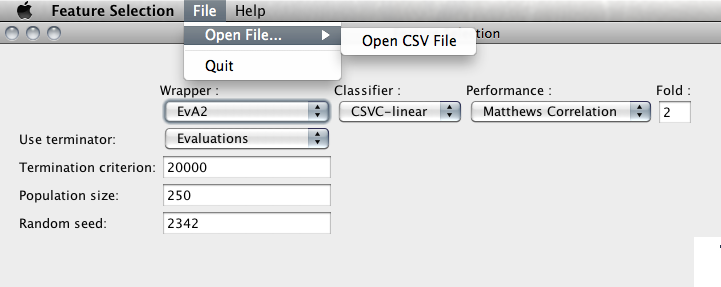
\includegraphics[scale = 0.4]{open.png}
\item Specify the wrapper, classifier, performance and fold to
  be used in this run.
\item If necessary, specify the parameters of EvA.
\item Start the selection by hitting the 'Start' button. 
\end{enumerate}

While the selection process is running you will not be able to start a new
one, however the running process can be forced to quit by clicking the
stop button.\\

Upon the start of the process two new windows appear : \\

~\includegraphics[scale = 0.4]{plot.png}

The left one, showing three tabs: results in a table, the graph, and a
description which holds the file name, the chosen settings an the final results.\\

The right window shows a graph depicting the results in a separate window.\\

The right result window holds a menu to save the plot as
.svg file, the
table as .csv file and the description as txt file.\\

~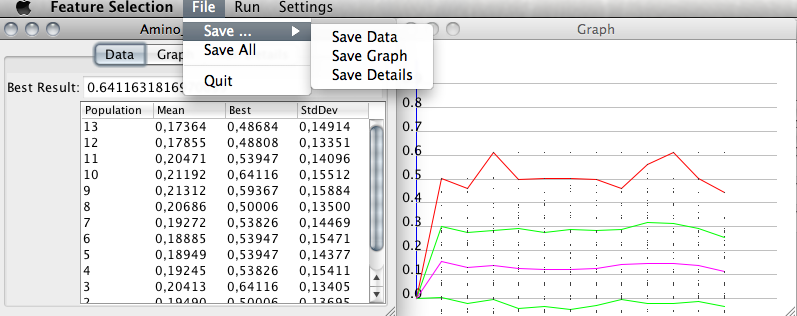
\includegraphics[scale = 0.5]{save.png}

Additionally you can set the visibility of the single curves in the plot. \\

~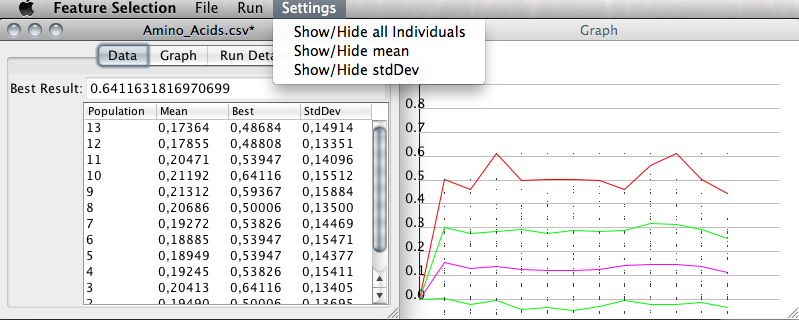
\includegraphics[scale = 0.5]{show.png}

\section{How to enlarge the feature selection API}

\subsection{Create a new wrapper}

To create a new wrapper you will have to create a class that extends the
abstract WrapperBase class. The parameters your new wrapper may need
can be stored in a config class that implements WrapperConfigBase.\\
After the implementation of a new wrapper class you will have to add the
new wrapper to the enum WrapperTypes. This will make it possible to choose the
new wrapper in the GUI, however if your wrapper requires parameters, you will have to update the GUI.

\subsection{Create a new performance}

If you would like to implement a new method to calculate the performance of
the binary classification you will have to create a new class that
implements the PerformanceI interface and implement its
calculatePerformance method. If you need to store parameters for your
performance class you can create a new config class that extends
PerformanceConfigBase. Add your new performance to the enum
PerformanceTypes to make it accesible via GUI.
 
\subsection{Create a new cross validation}

If you would like to implement another cross validation, 
create a new class that extends the CrossValidationBase class and 
implement all necessary methods. If you need to store parameters for your
cross validation class you can create a new config class that extends
CrossValidationConfigBase. 

\subsection{Create a new classifier}

If you would like to implement another classifier just create a new class
that extends the ClassifierBase class and implement all the methods
you need to.  If you need to store parameters for your classifier
class you can create a new config class that extends ClassifierConfigBase. Add your new classifier to the enum
ClassifierTypes to make it accesible via GUI.


\end{document}
